\chapter{Related Work}
\paragraph{}There are various kinds of studies and researches that are related to this project. This mainly involve Bluetooth Low Energy.

\section{Similar to our proposal}
\paragraph{} There have been multiple proposed methods and multiple technologies for indoors localization. However, most of them use the Bluetooth low energy (BLE) and WiFi technology in the research. Moreover, the Received Signal Strength (RSSI) is one of the most popular and common way to estimate the position. Thus, in this chapter, we present the related work that use BLE and RSSI with these techniques: solely RSSI in distance estimation, Triangulation, Fingerprint-based method, and Trilateration.


Received signal strength indicator (RSSI) is used to estimate the indoor position in \cite{ref:r10}. The observation in this research is done in a 10.5 meters x 15.6 meters room with 22 beacons installed around the room. The system determines the location by measuring which beacon has the highest RSSI value. The experiment achieved the correct estimation rate of 96.6 percent.

In [11], the authors introduced the three-dimensional positioning system using three-dimensional coordinates triangulation to calculate the position of each node and RSSI to measure the distance among beacons. The error rate from estimation is reduced by 27 percent from existed two-dimensional positioning system. 

Fingerprint-based method is another technique used in positioning system. In [12], the authors explored the use of BLE beacons for fingerprint positioning. The research was conducted using 19 beacons distributed around the approximately 600 square meters room. They achieve the tracking accuracies with 95 percent of the time containing an error less than 2.6 meters using dense beacon distribution (one beacon per 30 square meters) and less than 4.8 meters for lower density distribution (one beacon per 100 square meters) compared to the accuracy of error less than 8.5 meters achieved from the WiFi technology using the same method in the same environment.

In [13], the authors presented two post-processing filters (accuracy function and correction function) after applying the trilateration method to enhance the estimated result. The mean and standard deviation of the estimation are minimized after the post-processing filters are added, thus, they concluded that the trilateration method can be used in indoors localization and the post-processing filters are recommended to make the estimation more accurate.

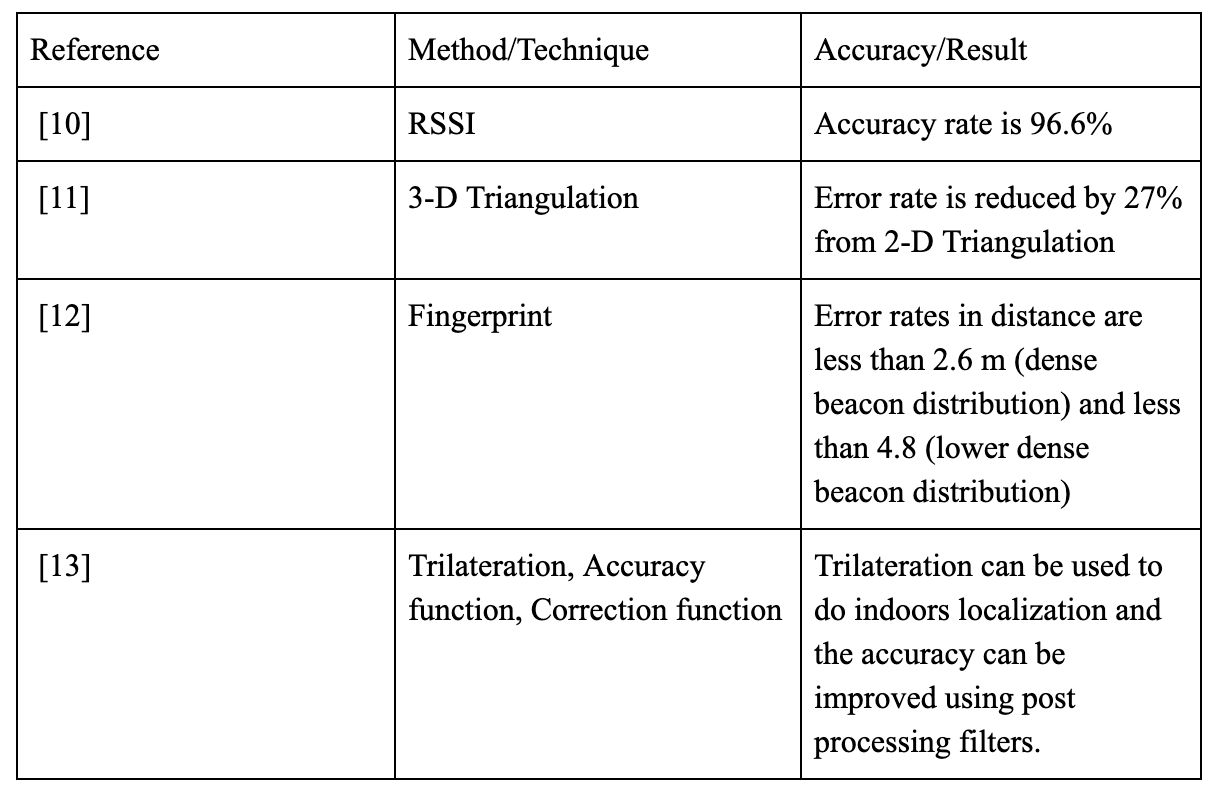
\includegraphics[scale = 0.6]{Image/tableofrelated.png}


\section{Studies with other technologies}
\paragraph{} Since GPS performs poorly in a building, different indoor positioning systems (IPSs) and technologies are studied in order to solve indoor positioning problems. Researches are carried out on different indoor localization methods and different technologies employed in indoor positioning systems. This section will describe several existing technologies used in the system to locate an indoor object. Gu and Lo’s survey [14] divides IPSs into six categories according to the technologies employed.

\subsection{Infrared Signal}
\paragraph{} Infrared signal (IR) [3] is electromagnetic wave with longer wavelengths than visible light, therefore, infrared is invisible to the human eyes. Infrared is generally used in commercial goods such as television, and air conditioner. Infrared that utilized for locating the object is called IR-base IPS. An example of IR-base IPS is use IR-base on incident angles of infrared emitters [6]. There are three infrared emitters on fixed known positions. An incident angle sensor measures the angle differences between each two emitters. Measured angle differences determine a position. The main disadvantage of IR-base IPS is the infrared as light wave cannot pass through opaque objects. From this problem, the object and emitters must be placed with no obstacles blocking the infrared signal.

\subsection{Radio Frequency}
\paragraph{} Radio frequency (RF) refers to an oscillation rate of electromagnetic radio waves. Radio frequency is used in various technologies such as communication, detection, or even researching. In term of indoor positioning system, technology types of radio frequency that utilized for detect the object are called RF-base IPS. The main feature of RF-base IPS is it passes through most of obstacles. Therefore, RF-base IPS can solve a line of sight propagation.

\subsubsection{Radio Frequency Identification}
\paragraph{} Radio Frequency Identification (RFID) [5] consist of tags and reader devices. This system is divided in two major type: active and passive. The RFID active system has a tag with battery inside, on the other hand, RFID passive does not. RFID enables identification from a distance, it does so without requiring a line of sight. The tags activated by reader device and return the information, such as product id, temperature. Using the RFID in term of indoor positioning is for tracking object or human, such as tracking patient in hospital, tracking product in supermarket.

\subsubsection{Ultra-wideband}
\paragraph{} Ultra-wideband (UWB) [2] is a RF technology that can use a very low energy level for high-frequency and short-range communications over a large portion of the radio spectrum. Ultra-wideband (UWB) uses broad frequency bands to allow transmission using high-energy pulses while limiting the interference with other RF equipment operating within the same frequencies. In term of IPS, UWB-based systems usually rely on time-based methods such as Angle of Arrival (AOA), Received Signal Strength (RSS) [8] to determine the position between reference node (UWB receiver) and the target node (UWB transmitter).

\subsubsection{Wireless local area network}
\paragraph{} Wireless Local Area Network (WLAN) [3] is a network in which a wireless
router communicates with several WLAN compatible devices such as smart phone, laptop, which mean no need unique additional devices. Using in the indoor positioning, WLAN-base IPS use RF signal for communication, therefore, the RSSI can be used in the same way as with RFID to get the distance to a user from an access point. It can also be implemented on top of existing Wi-Fi infrastructure. The problem of WLAN-base IPS is that the accuracy is very limited, thus it needs extra algorithms or hardware to compensate to ensure the good performance.


\subsubsection{Bluetooth}
\paragraph{} Bluetooth is wireless technology widely used in local positioning system (LPS). It works in short range and lower data transfer rate. Bluetooth Low Energy (BLE) provides portable battery-powered beacon at low cost and consume less energy. BLE is used in range-based indoor positioning system [15][16], location fingerprinting [17]. Due to its ultra-low power consumption the localization using BLE can have an error rate up to 5 meters. The Topaz local positioning system [18] is the newer generation of BLE-based IPS. It provides room wise accuracy of 2 meters. The further enhancement of Topaz system is to integrate it with infrared and other transducers, with the Bluetooth positioning capability.

\subsubsection{Wireless Sensor Networks}
\paragraph{} Wireless sensor network (WSN) is a group of sensors spatially dispersed for monitoring recording of environment and organizing the collected data at a central location. Each sensor node contains transducer, microcomputer, transceiver, and power source. The transducer generates electrical signals. Then the microcomputer processes and stores the output. The transceiver receives commands from a central computer and transmits data to it. WSN can be constructed using star, tree, or mesh topologies. It can be applied to many topics such as, open source API, iOS, and Android [19], and WSN-based localization system using trilateration and fingerprint method [20]. Both of the methods yield result with error less than 1.2 meters.

\subsection{Geomagnetic-field}
\paragraph{} Geomagnetic-field from earth is often used as navigator. The compass uses geomagnetic-field to find directions. There has been studies of indoor localization using magnetic field [21]. The geomagnetic-field based indoor localization suffers from a lot of fluctuation due to structure of the building which include steel, concrete, etc. These can make the data fluctuate. Assuming the anomalies inside the building is static, the magnetic fingerprint can be utilized in localization. In addition, the Monte Carlo localization has been proposed. Monte Carlo localization (MCL), is an algorithm for robots to localize using a particle filter. Given a map, the algorithm calculates the position of the robots as it moves. The research concludes that the deviation of magnetic field can be used in self-localization and that the ambient magnetic field may remain stable for longer periods of time.

\subsection{Ultrasound Wave}
\paragraph{} Ultrasound wave is a type of inaudible sound wave that can travel through air and solid materials. The use of ultrasound wave can be seen in bats. Bats emit ultrasound on an object and rely on the echo to navigate them in the darkness. Similar mechanism is used for indoor localization called the active bat system [4],  equipped with matrix of fixed reference nodes that act as ultrasound receivers on the ceiling. The tag worn by a person will emit ultrasound signal then the signals are captured by the receivers on the ceiling. The location of the person is then calculated by applying the time-based trilateration method. Unlike infrared light wave, ultrasound wave does not require line-of-sight propagation, so it can locate hidden objects.

\subsection{Geomagnetic-field}
\paragraph{} Geomagnetic-field from earth is often used as navigator. The compass uses geomagnetic-field to find directions. There has been studies of indoor localization using magnetic field [21]. The geomagnetic-field based indoor localization suffers from a lot of fluctuation due to structure of the building which include steel, concrete, etc. These can make the data fluctuate. Assuming the anomalies inside the building is static, the magnetic fingerprint can be utilized in localization. In addition, the Monte Carlo localization has been proposed. Monte Carlo localization (MCL), is an algorithm for robots to localize using a particle filter. Given a map, the algorithm calculates the position of the robots as it moves. The research concludes that the deviation of magnetic field can be used in self-localization and that the ambient magnetic field may remain stable for longer periods of time.

\subsection{Audible Sound}
\paragraph{} Audible Sound is sound wave that typically generated by human. Basically, it can travel through air, and solid object, medium is necessary for its travel. Audible sound wave can be emitted by every mobile devices such as mobile phones and laptops. The study of an indoor location system that senses audible sound state that sound is sensitive to noise, so the localization process that uses audible sound will be degraded by noise interference. A possible solution is to operate audible sound-based IPS in a small, quiet environment.

\subsection{Camera Positioning}
\paragraph{} The use of camera and computer vision technology for indoor localization is known as vision-based IPS [1]. In the studied, the micro-flyer equipped with two cameras take pictures of the special texture on the wall. By analyzing the distortion of the captured texture, the system can estimate its relative locations from the walls. The UAV (Unmanned Aerial Vehicle) [7] shots laser beams to the surrounding. By capturing and analyzing the position of the laser points on the walls and ground, the UAV can predict its distance from ground and walls. However, vision based localization consumes significant amount of power and computing resources that are used to analyze the captured image. Furthermore, the use of camera will increase the cost of the system results in low scalability
    
